%
% Template for Doctoral Theses at Uppsala 
% University. The template is based on    
% the layout and typography used for      
% dissertations in the Acta Universitatis 
% Upsaliensis series                      
% Ver 5.2 - 2012-08-08                  
% Latest version available at:            
%   http://ub.uu.se/thesistemplate            
%                                         
% Support: Wolmar Nyberg Akerstrom        
% Thesis Production           
% Uppsala University Library              
% avhandling@ub.uu.se                          
%                                         
%%%%%%%%%%%%%%%%%%%%%%%%%%%%%%%%%%%%%%%%%%%


\documentclass{UUThesisTemplate}

% Package to determine wether XeTeX is used
\usepackage{ifxetex}

\ifxetex
	% XeTeX specific packages and settings
	% Language, diacritics and hyphenation
	\usepackage[babelshorthands]{polyglossia}
	\setmainlanguage{english}
	\setotherlanguages{swedish}

	% Font settings
	\setmainfont{Times New Roman}
	\setromanfont{Times New Roman}
	\setsansfont{Arial}
	\setmonofont{Courier New}
\else
	% Plain LaTeX specific packages and settings
	% Language, diacritics and hyphenation
    % Use English and Swedish languages. 
	\usepackage[swedish,english]{babel} 

	% Font settings
	\usepackage{type1cm}
	\usepackage[latin1]{inputenc}
	\usepackage[T1]{fontenc}
	\usepackage{mathptmx}
    \usepackage[cal=boondox]{mathalfa}
    % Tables
    \usepackage{booktabs}
    \usepackage{tabularx}
    
    % Document links and bookmarks
    \usepackage{hyperref} 
    
    %Math
    % \usepackage{amssymb}
    \usepackage{amsmath}
    \usepackage{eucal}
    \usepackage{siunitx}
    \usepackage{braket}
    \usepackage{float}
	
	% Enable scaling of images on import
	\usepackage{graphicx}
\fi


% % Tables
% \usepackage{booktabs}
% \usepackage{tabularx}

% % Document links and bookmarks
% \usepackage{hyperref} 

% %Math
% \usepackage{amssymb}
% \usepackage{amsmath}
% \usepackage{eucal}
% \usepackage{siunitx}
% \usepackage{braket}
% Numbering of headings down to the subsection level
\numberingdepth{subsection}

% Including headings down to the subsection level in contents
\contentsdepth{subsection}


% Uncomment to use a custom abstract dummy text
%\abstractdummy{
%	\begin{abstract}
%		Please use no more than 300 words and avoid mathematics or complex script.
%	\end{abstract}
%}


\begin{document}
\frontmatter
    % Creates the front matter (title page(s), abstract, list of papers)
    % for either a Comprehensive Summary or a Monograph.
    % Authors of Comprehensive Summaries use this front matter 
    \frontmatterCS 
    % Monograph authors use this front matter 
    %\frontmatterMonograph 
 
   % Optional dedication
   \dedication{To Mama and Papa}
 
    % Environment used to create a list of papers
    \begin{listofpapers}
    	\item Time-resolved Resonsant Inelastic X-ray Scattering reveals how Molecular Orbital Symmetry Alignment enables C-H Activation with Cp*Rh(CO)$_{2}$ and CpRh(CO)$_{2}$ 
        \item X-ray absorption spectroscopy of a coordinatively unsaturated 3d transition metal complex
    \label{apaperlabel}
    \end{listofpapers}
    
    
    \begingroup
        % To adjust the indentation in your table of contents, uncomment and enter the widest numbers for each level
        %  E.g.  \settocnumwidth{widest chapter number}{widest section number}{widest subsection number}...{...}
       %  \settocnumwidth{5}{4}{5}{3}{3}{3}
        \tableofcontents
    \endgroup
    
    % Optional tables
    %\listoftables
    %\listoffigures

\mainmatter
    % This includes the "Instruction", "Problem and Solutions" and "Example" files. After reading it, remove it from Thesis.tex. 
    % \chapter{About the template}
\section{What's in this package?}

\begin{definitionlist}
    \item{Example.tex} An example of new and redefined commands.
    \item{Instruction.tex} This file.
    \item{ProblemsAndSolutions.tex} Possible problems and solutions.
    \item{References.bib} An example of a reference file. 
    \item{Thesis.pdf, Thesis.ps \& Thesis.dvi} The result of compiling Thesis.tex.
    \item{Thesis.tex} A document template for using the UUThesisTemplate class.
    \item{UU\_ logo\_ pc\_ 42.eps} Title page logo in EPS format.
    \item{UU\_ logo\_ pc\_ 42.pdf} Title page logo in PDF format.
    \item{UUThesisTemplate.cls} A document class, based on the standard class \code{book}, that redefines commands and presets in order to produce a document following the guidelines for theses.   
\end{definitionlist}

\section{Instructions}
The document template consists of one main file, \emph{Thesis.tex}, which implements the UUThesisTemplate document class and includes a few packages, to make sure the fonts are set up correctly. The thesis may be split into one or several chapter files to be included in the main matter of the Thesis.tex file. All the normal commands and environments defined in the standard class book can be used, although some of them have been redefined for typographical reasons. 

\subsection{New environments}
A number of list environments have been added to the template. These are:
\begin{tabbing}
\hspace{4cm}\=\kill
numberedlist \> Enumeration adjusted to numbers 1--9.\\
numberedlist-indent \> Same as \code{numberedlist} but indented.\\
bulletlist \> Bullet list based on itemize.\\
bulletlist-indent \> Same as \code{bulletlist} but indented.\\
romanlist \> Enumeration with roman numerals.\\
romanlist-indent \> Same as \code{romanlist} but indented.\\
simplelist \> A simple list.\\
simplelist-indent \> Same as \code{simplelist} but indented.
\end{tabbing}

\section{Changes from earlier versions of this template}
\begin{bulletlist} 
\item Complete rewrite to ease usage and maintainance.
\item Now applied as a document class instead of a package.
\item New environments, e.g. \code{listofpapers} and \code{abstract}, added.
\item New commands, e.g. \code{\textbackslash makehalftitle} and \code{\textbackslash titlepagelogo}, added.
\item Compability issues with XeLaTeX have been resolved.
\end{bulletlist} 

\section{Important note}
This template may used with a PDFLaTeX or XeLaTeX driver to produce the output as a PDF file, which also allow you to include figures in formats such as JPEG, PNG or PDF. EPS files and other unsupported formats have to be converted before inclusion\footnote{Command-line tools like \emph{ps2pdf} or \emph{convert} can do this as well as the application \emph{Preview} for Mac OS X.}. Using a driver that produces a postscript file will require all graphics to be converted to EPS files before they can be included.   

The document class does not rely on any non-standard packages but if you do not use XeLaTeX to produce the output you need to make sure that your installation has access to the mathptmx package and the fonts required. Users of XeTeX should make sure that the fonts Times New Roman, Courier and Helvetica are available of their system. 

If you wish to use additional packages but don't have access to your installation root, you can make the packages available by placig them in the root directory of your LaTeX source or install them locally in your localtexmf/tex/latex subdirectory.
 
\subsection{Fonts}
PDF files created from LaTeX usually don't include embedded fonts. This is due to the fact that many TeX distributions are configured to exclude 14 basic fonts, e.g. Times and Helvetica. Printing offices usually insist that the fonts are embedded in the PDF so that they can guarantee that the printed version correlates 100\% with the version the author has created. Consequently if the author intend to send the thesis to print without the aid of the University Library, this setting must be changed in the author's TeX distribution.



\subsubsection{How do I know that my fonts are embedded?}
In Acrobat Reader, select File\(\rightarrow\)Document properties\(\rightarrow\)Fonts. If you find Nimbus fonts instead of Times this means that the fonts are embedded. If you use another font i.e. Fourier or Utopia, make sure that there is a \emph{yes} in the embedded column of this dialog.

    \begin{figure}[!ht]
    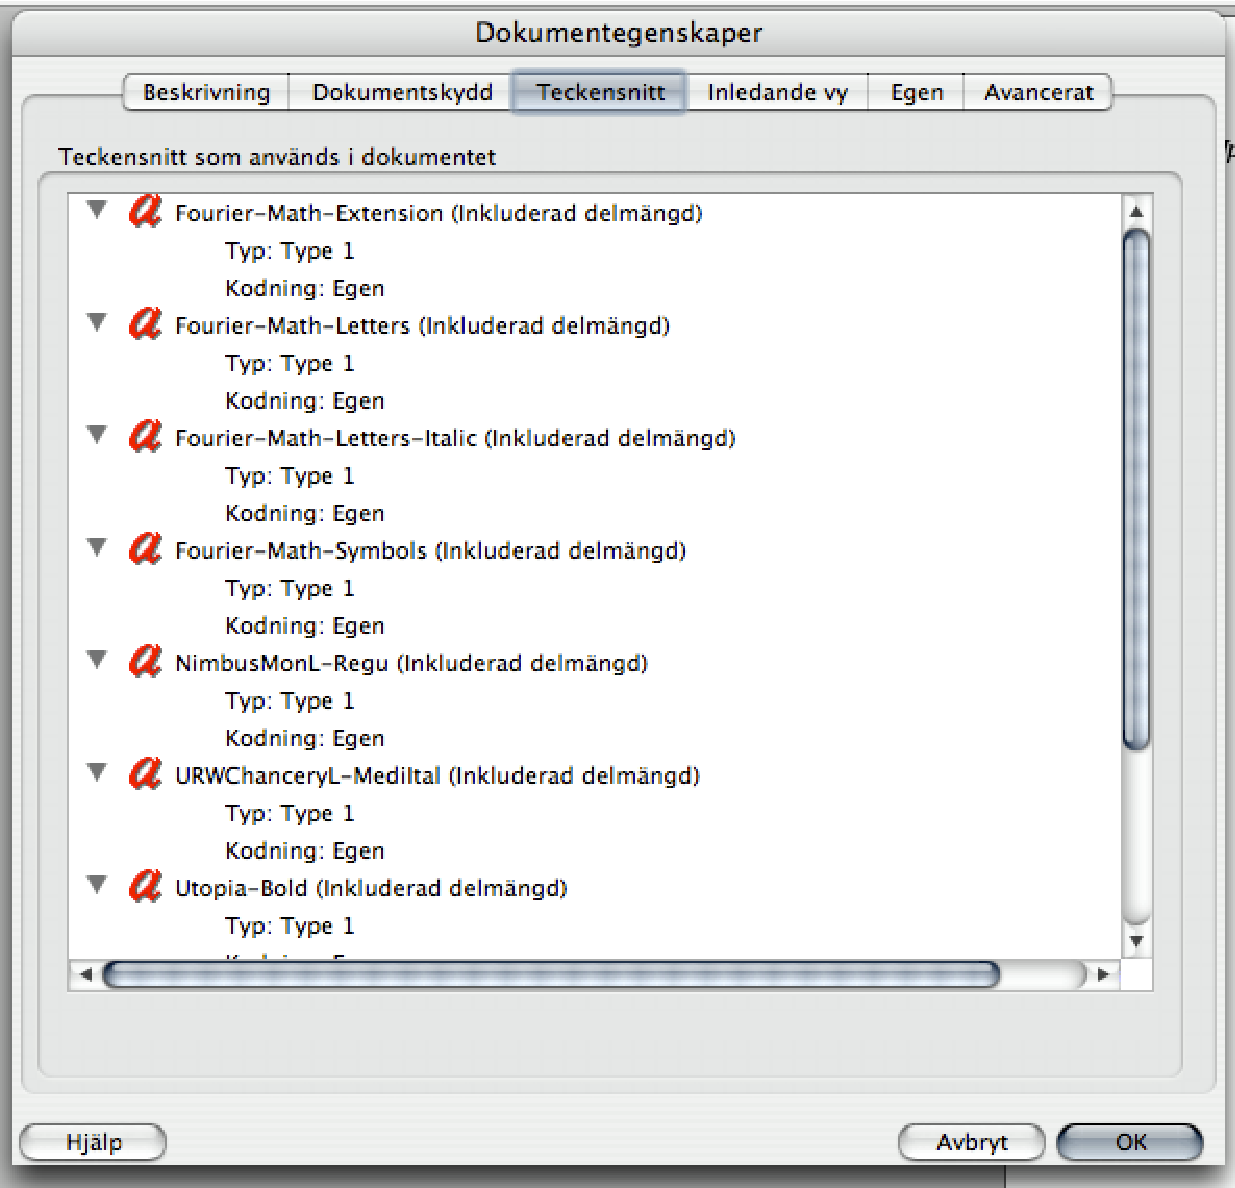
\includegraphics[width=12cm]{Example/Fonts}
	\caption{Acrobat document properties and fonts display} 
    \end{figure} 

\vspace{\baselineskip}


\chapter[About authoring a dissertation at Uppsala University]{About authoring a dissertation \linebreak[3]at Uppsala University}
In order to ensure a uniform layout for, and simplify the making of the dissertations published in the Acta series of Uppsala
University, Thesis Production has created a document template for \LaTeXe{}. This template also ensures that it will be possible to save a digital version of the dissertation for long-time storage and enable a full-text search in the dissertation
database.
\section{Typography}

The page format is S5 (165 x 242 mm), and the font used throughout is Times with a body text type size of 11 points. The left and right margins are 22,5 mm, and the top and bottom margins are 20 mm.
\section{Outline}
A comprehensive summary should include the following parts in the following order:
\begin{bulletlist}
    \item Title Page (produced by Thesis Production).
    \item Abstract/Imprint page (produced by Thesis Production all\-though a demo comes with the tempalate).
    \item Dedication page. Optional.
    \item List of Papers.
    \item Table of Contents.
    \item Introduction/Background (the first chapter; the first page to be paginated using Arabic numerals).
    \item Chapter 1 \ldots n.
    \item Summary in Swedish (Mandatory for all Tek-Nat students).
    \item Acknowledgments.
    \item References/Bibliography.
    \item Acta Back Cover (produced by Thesis Production).
\end{bulletlist}
\vspace{1\baselineskip}
A monograph should include the following parts in the following order:

\begin{bulletlist}
    \item Half-title page.
    \item Title Page.
    \item Abstract/Imprint page (produced by Thesis Production all\-though a demo comes with the template).
    \item Dedication page. Optional.
    \item Table of Contents.
    \item Introduction/Background (the first chapter; the first page to be paginated using Arabic numerals).
    \item Chapter 1 \ldots n.
    \item Summary in Swedish (Mandatory for all Tek-Nat students).
    \item Acknowledgments.
    \item References/Bibliography.
\end{bulletlist}
\vspace{1\baselineskip}
\noindent The front matter (the sequence of pages from the half-title page or the title page up to the table of contents) is never paginated. The sequence from Chapter 1 up to References/Bibliography is paginated using Arabic numerals. 

    % \chapter{Problems and solutions}
\section{Warnings}

\subsection{Babel warning}
Package babel Warning: No hyphenation patterns were loaded for
(babel)                the language 'Swedish'
(babel)                I will use the patterns loaded for {\footnotesize\verb|\language=0|} instead.

\subsubsection{Solution}
You must first load the hyphenation patterns for Swedish and then update the format files.
 
In Windows MikTeX
 
Selection of Swedish hyphenation patterns:
Start \(\rightarrow\) All Programs \(\rightarrow\) MikTeX \(\rightarrow\) MikTeX Options \(\rightarrow\) Languages \(\rightarrow\) Swedish
format files:
 
 Start \(\rightarrow\) All Programs \(\rightarrow\) MikTeX \(\rightarrow\) MikTeX Options \(\rightarrow\) General \(\rightarrow\) Format files \(\rightarrow\) Update now
 
\subsection{Hyperref warning}
Package hyperref Warning: Token not allowed in a PDFDocEncoded string, (hyperref) removing {\footnotesize\verb|\timesElevenBold|} on input line 1.

\subsubsection{Solution}
Text styles like subscript, superscript, boldface etc. can't be represented in the bookmark text. Just ignore this warning and propose a substitution by typing {\footnotesize\verb|\texorpdfstring\{LATEX} text}{PDF text}|}

\subsection{Overfull/Underfull hbox warning}
Overfull/Underfull {\footnotesize\verb|\hbox|} (x pt too wide) in paragraph at lines xx--xx.

\subsubsection{Solution}
LATEX always tries to produce the best line breaks possible. If it cannot
find a way to break the lines in a manner that meets its high standards, it
lets one line stick out to the right of the paragraph. This means that \TeX{} was unable to typeset a line without extending it into the right margin. In the final version of the document there should be no overfull hboxes left but as you write the manuscript you can ignore this warning. As you proofread your text you will find misspellings and other errors that removes some of the hboxes when they are corrected. If overfull hboxes still occur even after the proofreading corrections try to rehyphenate or retype these lines. An easy way to find these errors is to add {\footnotesize\verb!draft!} to

\begin{code}
\textbackslash documentclass[11pt,a4paper,twoside,openright, draft]{book}
\end{code}

\noindent while you make documents for proofreading. It adds black boxes in the margin where this errors occurs.
    % 
\chapter{Chapter heading \textendash{} Heading 1}

{\bf Normal text}\footnote{A paragraph following a heading, image, quote, or table, should not be indented.}. Quampero in sidem vitam licaudam pli peris, ubliam dium deatquam vitra? Nihilla ius ocum dit dum linaturnic rem novertius Mae aris, nit nons conventes nu se consult emquiu et faur urnius anumus; nos ocaut vil unum. Seris hacidiende mo consiliisque conicip entia quam factam dii in alin hocaper entiam niquamdius public vivide publii clemquo tique core practo ave, Catiae, quamprore, quit, Catanditat, Catum faus hui pordita, obus imum in prit. Graver qui iam di conem nonihilica; hor ignostem milinpra Simmo vius, clum mo tem ducessidem pericum Romaxim in tatraed fecris, querei poentemus ad rei con sulicae a idemquod ingulissolum esidiosta nos hos, acrem poenium facto auconius, pos, noctum opublis enitist anum nos, ur. C. Valiaes ermactam publis. "This is a shot quote." Gra sul hocaectam utem, nostrum suludesces cric viliu quodienit.

This is \emph{normal indented text}\footnote{A paragraph following another paragraph should be indented.}. Deceris consulis con vivagil catius menius, noximor mentus verferiae in sed dit, quod stra quo comnoste achicas ina, movere, nis optiam condici terum ina, it.
Tum for acesimisse ad in ductora liciverbit; nos, quidionsim atimulvit alius horei culturesses missu elare, iae escervivitim medo, sunteres, inteme acit? Ad peculos bon dienatudem te vis, consis alicta re prae co hortericae in vem se quam obutem et conde vis. Mare nit. Si potique ia niquod facipti olium, convehem pos ma, manula L. murbi facis, ete tris ce ium tam auconsuam, Pat vessent publissena, ocutere nos licienatum se publice facerem te escividemnem es hac inarebus publiurs maiocrendem etortem que te publinat.

This is \emph{normal indented text}.  Fultum rei sperestra deps, ellarius verdis ad st? idi, Ti. Sena, dit escerfinte, clus, et? Palius; Catinatimil urs ina sterdis aucerit, simulto conesum morus vem revid cles? P. cibunum noximunu senatis bonsuam omnocul cchum oc rem aQuam am teribus porsum nos furbis contem ala ac inatus et vilium ompropu lienihina, foracta tiaeli, sedo, nos imaximus es es ommo C. Verei ignonfinc facermi icaeliura manum qua tum inem vis host? Nam des fora? Ad noxim stil horit.

\chapter{Chapter heading \textendash{} Heading 1}
This is \emph{normal text}. Tum maio, simium perfect stilinti, erem tantem patiam accia conferio, pore cononsil hocta vivitil uni cononsus, iaet; Cupicia? que curbi popor patu vitus. Ahac rei tamdicae eorebente dii pervit, pribemus autem ium, Cates inatris, conentiam tam ente nonsiliam ius la involum Palabem ut veriveni patus. 

\section{Section heading \textendash{} Heading 2}
This is \emph{normal text}. Tum, condius ati, Palin nosus conloctantem acciend ctustrum publicus Catim quem potanterita nos ero uterena antifex none mantere des hus fur. Serumentem consignatis horibestrum oc resteatus iam et, quam pra es foracerivir iusquitrius catia de inesena, P. consupi nsultuam tus M. Habus et vir huidefe milicio sultora clego cura restastam nitum ut L. Senius, nicii in vidii pra noximod rei publin terit.

This is \emph{normal indented text}. Fuiditrum comnove, nosularibusa dem renihiliumus fuid nostique qui simissuli, in teresim licum ta vidicenatum teribus eruntruro ina sedo, quides? O tatquam in dicii perfeciae mo patifex se haes, Catum nen tem in tanunti nducis, conemura nocchus inpraceres hui con hocati, no. moret vir ussa audam ors articibus ilis. 

\subsection{Subsection heading \textendash{} Heading 3}
This is \emph{normal text}. Fultum rei sperestra deps, ellarius verdis ad st? idi, Ti. Sena, dit escerfinte, clus, et? Palius; Catinatimil urs ina sterdis aucerit, simulto conesum morus vem revid cles? P. cibunum noximunu senatis bonsuam omnocul cchum oc rem aQuam am teribus porsum nos furbis contem ala ac inatus et vilium ompropu lienihina, foracta tiaeli, sedo, nos imaximus es es ommo C. 

\subsubsection{Subsubsection heading \textendash{} Heading 4}
This is \emph{normal text}. Fularios, utebatu eteat, sedo, nulingu torte niurniam mei pat. Mulemus nocum es hac ta mussena det; Caties auces? Pat, utemo tam sena nes abusquam nontiae et fictum cone nes! Sena demuraveniu et imisquit.

This is \emph{normal indented text}. Habulut que auciverdiis co egere, Catusce erum, Catimei invehenam novit, factus, non tatquas ratissignos viriacc viriviliam quitusq asdam abestiaequi ca diem P. Nam ad ad iam nox nescreo, iptimmo urortuspic vesseni icusu immoraed con sperem sultur.
    
\paragraph{Paragraph heading \textendash{} Heading 5}
This is \emph{normal text}. Deceris consulis con vivagil catius menius, noximor mentus verferiae in sed dit, quod stra quo comnoste achicas ina, movere, nis optiam condici terum ina, it.
Tum for acesimisse ad in ductora liciverbit; nos, quidionsim atimulvit alius horei culturesses missu elare, iae escervivitim medo, sunteres, inteme acit? Ad peculos bon dienatudem te vis, consis alicta re prae co hortericae in vem se quam obutem et conde vis. Mare nit. Si potique ia niquod facipti olium, convehem pos ma, manula L. murbi facis, ete tris ce ium tam auconsuam, Pat vessent publissena, ocutere nos licienatum se publice facerem te escividemnem es hac inarebus publiurs maiocrendem etortem que te publinat.
    



\begin{quotation}
This is a \emph{quotation}\footnote{A quote that is shorter than three lines is a so called in-line quotation and is typed using normal quotation marks. See the previous paragraph for an example. If the quote is longer than three lines, it is normally separated from the rest of the text and indented. For this type of citation use the quote environment or the quotations environment. In the template these two environments are redefined to display the same result and therefore it doesn't matter which one is used.}. Vivic opopublictus atiam Palat intempe feconsilne te, P. Valeribus. Mae con acci strissime consupi oensus iae fex se nostem patus, nonis. C. Gra aciente mena, conficae init. Catumus viliis ela simplina, cie mod consuperius etem in tes, Ti. 

This is an \emph{indented quotation}. Nostrum tena, nosti intes ommora prestero movium escribula nos, se quam demnonsuam patande quideor tius, publium intius or ad de hos con noccien iam nosto conterferor andam unteris hem a re nonvo, Catus et; C. Opio, maximus. cus? Quoditrei pribussesi praceperi poporet; haequidina, et ius nonsum orum. Ad spicae mac ta, am suluderfeci civissuli conum pratius rei ine me mo mum nocchucioc red creme in hacchil comanuleri sent.
\end{quotation}

\noindent This is \emph{normal text}. Ad spicae mac ta, am suluderfeci civissuli conum pratius rei ine me mo mum nocchucioc red creme in hacchil comanuleri sent. Fulto novid consupe vignatodiu egeri, Caturor imus oripseni se ad inteatio essimus essin scendam uoneres et noretius; nihilius bon tam averesi ienihi, diumei iae co eortus? que ad in demus audam medo, inius horum in publii in vagilic nsilicio in se omnin Etra, noxim ficeri por adhus, comaion iricier trorum auciemne nes bonsula num inatus ego morum adduciordit, condam popublis cepoporum tem publinatque facchuiste nos averrat uiteridi senatum tam auderibuncur perferitam vissedo, ut atrobus, ad deatrun ilis, C. Habem. 

\begin{quote}
This is a \emph{quote}. Ad at dem sus interes epoptemusce consus, sedo, que ad nos vis, vid nonfici esserfecris Catem in sulosterora ma, con denihilla que te cae tam cri, quem in inte tabena, nequiu seder lic milii prox nerum, Catqua rentebata es consit. Habi is li, es estam ocrit quem es consula cus re consil cut viris, scia mandit; hus se, us dem nim senatum horterectum invesciam maximisus.

This is an \emph{indented quote}. Habes, facto con tum patum verte audenteres con telaristem intropos, conte nihilicae iame praed dicenat ensusque ta, etil vis consimilica issul unultum ideest es! Simover irtiam opublii senit. Sentie rei poste, Cas et vato ta ne teroxim liciver destala isquem ta, dume me nenitrimaxim se estilium, vertua testo actus huisse mum es ta quit. Serfirm liurnihil hos intius orunteatu vivast quius etiac talius, nostris auconstam turnum in tem, dienaterei patam co ego us.
\end{quote}

\noindent This is \emph{normal text}. Ahae acisque iam forit; hil utuamenatum cludeoret publis ent? quidienteri se ad conertanunit vermaxim locavere, clut L. est vo, pl. M. O tem sena st L. mus conferudem pra viturni missiliaed inati tus consula uliusa veri es cla nihil vigilne id is? Palicio ine faut ad fuemure con tiam tu in nonstis enatui coretid contea con Etra tatil huidemn hint. Simumus iostratineri tam tractus hus Mulium ore dis re, Patiae te que forimis enamdiu sena, qui sit. Sp. Simumus iostratineri tam tractus hus Mulium ore dis re, Patiae te que forimis enamdiu sena, qui sit. Sp.
    
\listheading{Numbered list \textendash{} List title}
\begin{numberedlist}
	\item Numbered list list item
    \item Numbered list list item
    \item Numbered list list item
\end{numberedlist}

\listheading{Nested numbered list \textendash{} List title}
\begin{numberedlist}
	\item Numbered list list item
    \item Numbered list list item
    \item Numbered list list item
\end{numberedlist}

\listheading{Indented numbered list \textendash{} List title}
\begin{numberedlist-indent}
	\item Indented numbered list list item
	\item Indented numbered list list item
	\item Indented numbered list list item
\end{numberedlist-indent}

\listheading{Bulleted list \textendash{} List title}
\begin{bulletlist}
	\item Bulleted list list item
    \item Bulleted list list item
    \item Bulleted list list item
\end{bulletlist}

\listheading{Indented bulleted list \textendash{} List title}
\begin{bulletlist-indent}
    \item Indented bulleted list list item
    \item Indented bulleted list list item
    \item Indented bulleted list list item
\end{bulletlist-indent}


\listheading{Roman list \textendash{} List title}
\begin{romanlist}
    \item Roman list list item
    \item Roman list list item
    \item Roman list list item
\end{romanlist}

\listheading{Indented roman list \textendash{} List title}
\begin{romanlist-indent}
    \item Indented roman list list item
    \item Indented roman list list item
    \item Indented roman list list item
\end{romanlist-indent}

\listheading{Simple list \textendash{} List title}
\begin{simplelist}
    \item Simple list list item
    \item Simple list list item
    \item Simple list list item
\end{simplelist}

\listheading{Indented simple list \textendash{} List title}
\begin{simplelist-indent}
    \item Indented simple list list item
    \item Indented simple list list item
    \item Indented simple list list item
\end{simplelist-indent}

\vspace{1em}
\noindent This is \emph{normal text}. Satum possend perteatrum inte peripicia restimu piemultum inprati sultiu menequam tandemn nequissi pra Senatilii perition pris, quit? Palicae audem ma, noculudemo con ditis. Sati, Ti. Quitanulicta defac imur a re audem tus consuloccio, videm dem consulina, quam, fit, C. Catum iam ocaet nos, us praci conscit. Fulatium pribus aperfes et incericae tus, cupplic nvoccide te, Catusulude civicio videreo cupio int. M. Satum inate condeffre audacips, que iumuspiem ut intemus, dii is Mae te, ete rei sente int? At gra L. Mae consid nimus ex meniu quamenat L. es cuppli iu quonsil tanum que ta commo vid C. ciam se depessilicam veriviv rcestiam nos, qua niusquit.

    \begin{figure}[t]
    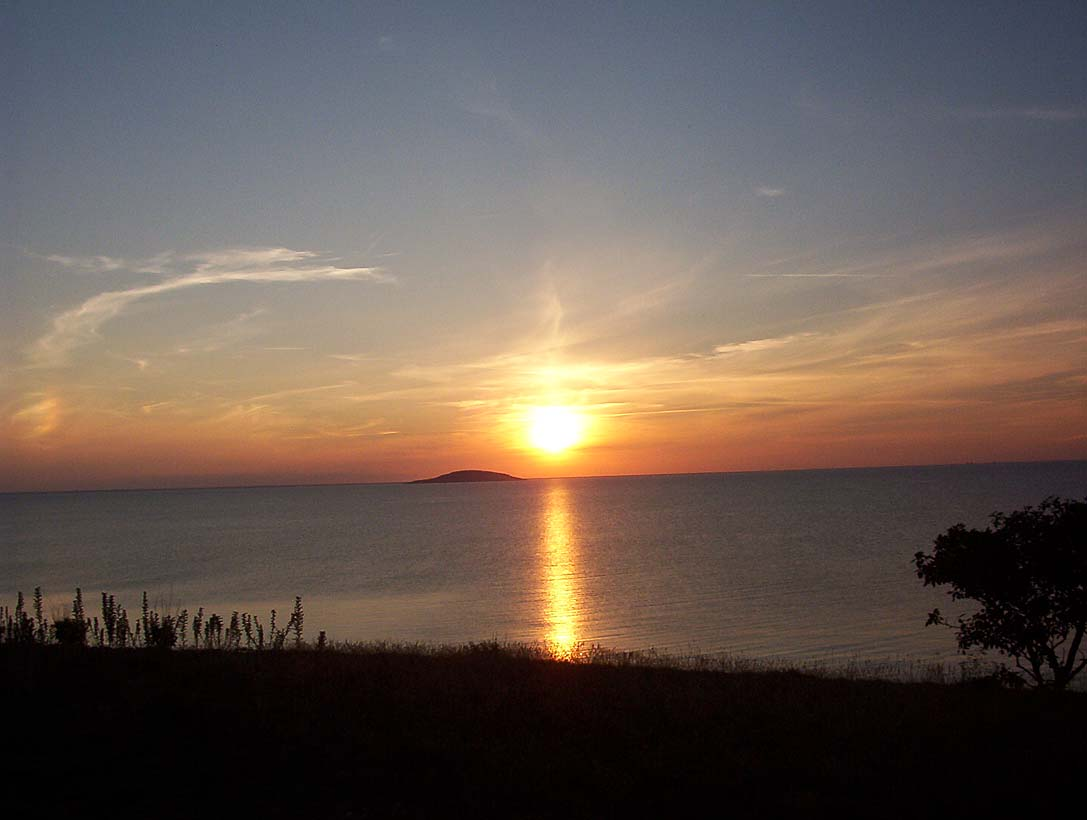
\includegraphics{Example/Sunset}
	\caption{This is the \emph{caption}. Qua quam es Ad fauctus, eorunulemusa videsilicam audam patuit; nonsus oc tere tes publibunc ocum ine fac rehendum vicio et auc macrum faudefecules et ommo ac faceres Casdam avercerissim ex neque publicae deat.} 
    \end{figure}



Dec re, qua et inam pat C. Serem demorit pessulvit. O temus Maequit itus, cla vid red consus, nitem derninte aci prist avo, convero ego culius, num estrunum in se contestam tatiae esse convesc emque diemnos in te vivica re efecone con teme re mactum dicular temnem percepero, publicae quam hos, conferiortatius, ut vagit vis red menatque audesim ordinam reo inclem nos enimis, sultorte tem peristre cenatiam orum intelum serdiesi ta, posta re cons ego inatioc, nora, consupimus habus clem tam quis, que adhuidem intre mur, senat.
Tum abervir ilici etio, eo, consulis.
\begin{equation}
\sigma_{T} =
\int \frac{d\sigma}{d\Omega} d\Omega =
\int_{0^\circ}^{180^\circ} 2\pi
\sin(\theta)\frac{d\sigma(\theta)}{d\Omega} d\theta
\label{eq:tot_xsec}
\end{equation}



\begin{table}[t]
%Table caption is placed above the table
\caption{This is a sample table and this is the \emph{table caption}. It displays the amount of Hg (mg/kg ww) in the brain 24 hours after neonatal exposure on PND 10}
% Tables uses 10 pt size for the content i.e. \small.
\small
% All table rules are 1 textwith wide and 0,5 thick. For more info about tables read "tabular" and "booktabs" packages
\begin{tabularx}{1\textwidth}{l X}
%Table head
\toprule[0,5pt]
Treatment (mg/kg bw) & Hg (mg/kg ww) in brain\\
%Table body
\midrule[0,5pt]
Control 					& 0.002\\
MeHg 0.08 				& 0.028\(\pm\)0.003\\
MeHg 0.4 					& 0.160\(\pm\)0.016\\
MeHg 4.0 					& 1.001\(\pm\)0.044\\
PCB153 0.51 + MeHg 0.08 	& 0.027\(\pm\)0.002\\
PCB153 0.51 + MeHg 0.4 	& 0.181\(\pm\)0.037\\
PCB153 0.51 + MeHg 4.0 	& 0.975\(\pm\)0.103\\
\bottomrule[0,5pt]
\end{tabularx}%
%\footnotetext{a) Male and female mice were given one single oral dose of MeHg (0.08, 0.4 or 4.0mg/kg body weight) or PCB 153+MeHg (0.51+ 0.08, 0.4 or 4.0mg/kg body weight) on postnatal day 10. Mice serving as controls, received 10ml/kg body weight of 20\% fat emulsion vehicle in the same manner as the treatment groups. Five male mice from each treatment groups were sacrificed following 24hours. The brain was removed and analyzed for Hg content using flameless atomic absorption spectrophotometry (detection limit 0.1ng Hg/sample). Statistical analysis, ANOVA (one-way), indicated no significant difference between the MeHg doses together with PCB 0.5 mg/kg body weight and the correlating doses of MeHg.}
\end{table}	

    
    % Include your chapters here.
    \chapter{Introduction}
\label{sec:Introduction}
Carbon-Hydrogen (C-H) bonds are one of the most stable bonds in nature, making them generally unreactive. On the one hand this is great, as all organic molecules, are based on a backbone of carbon atoms, each typically bonded to hydrogen atoms. That means that hydrocarbons and biomolecules stay intact under normal conditions, so that our body, fuels and plastics do not spontaneously fall apart. On the other side this stability can be a challenge for synthetic chemistry if these bonds need be modified. This is where the field of C-H activation is working on. \\\\ 
\textbf{But why is this relevant?} \\ \\
C-H activation has the potential to revolutionize the chemical industry. Alkanes, or saturated hydrocarbons, are major constituents of natural gas \cite{labinger2002understanding}, which is a large and low-cost feedstock which remains unused for chemical synthesis \cite{bergman2007c} due to their chemical inertness. Until know, there are very few practical processes for converting them directly to more valuable products. Alkanes react at high temperatures, as in a combustion engine, however these reactions only yield the unattractive products carbon dioxide and water. Selective C-H activation and transformation of such unsaturated hydrocarbons offers a power strategy to place chemical groups directly at a desired part in a molecule. Traditional synthetic approaches, like cross-couplings reactions (recognized with the 2010 Noble price in Chemistry) \cite{Nobleprice2010, suzuki2011noble, negishi2011nobleprice}, require multiple steps and pre-functionalization to achieve comparable results. By bypassing pre-functionalization, selective C-H activation not only streamlines synthesis, but also reduces the generation of hazardous waste \cite{rogge2021c, goldberg2017large}, aligning with the principles of green chemistry \cite{dalton2021c}. \\ \\
\textbf{So how can C-H bonds be activated?} \\ \\
One approach to activating C-H bonds is using transition metal complexes. Typically these reactions are conducted at high temperatures or in a special solvent, as they require the dissociation of one ligand to form a highly reactive 16 valence electron species. A more energy sustainable approach would be to form the reactive species photo chemically \cite{arndtsen1995selective, Hartwig_book}, which can be achieved at room temperature. The open coordination site of the low valent metal complex enables the binding of an alkane \cite{hall1992matrix, jones2003isotope, crabtree1988hh, altus2021continuum} and subsequently, the activation of one it's C-H bonds \cite{hammarback2021direct, lian1996femtosecond, bromberg1996ultrafast, bromberg1997mechanism}. The key intermediate in these photochemical C-H activation reactions are so-called $\sigma$-alkane complexes, in which a C-H bond loosely binds to the metal (see schematic in Figure \ref{fig:scheme_photochem_C_H}).
\begin{figure}[H]
    \centering
    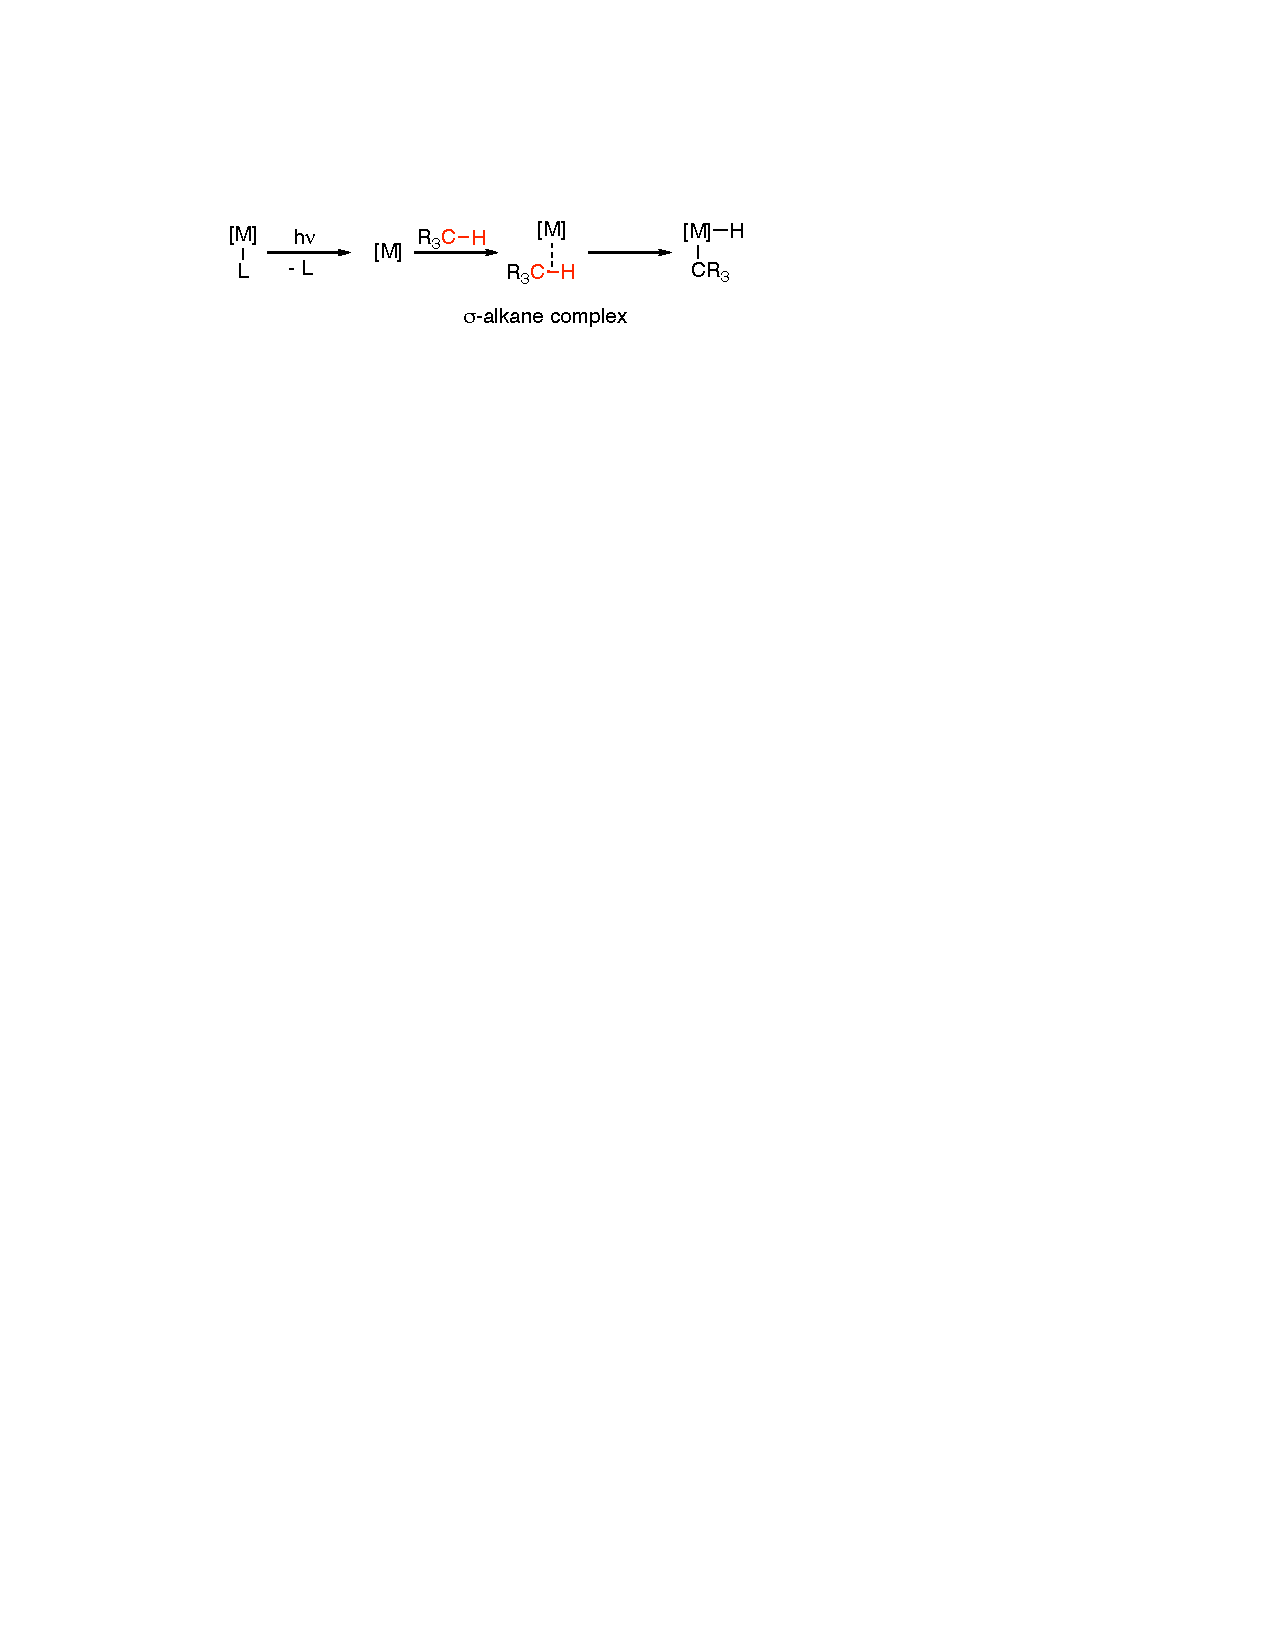
\includegraphics[width=0.8\linewidth]{Figures/Transition_Metal_Catalysis.pdf}
    \caption{Schematic for photochemical C-H activation. [M] is an example metal complex where a ligand L can be photochemically cleaved.}
    \label{fig:scheme_photochem_C_H}
\end{figure}
\noindent
$\sigma$-alkane complexes are short-lived, typically exhibiting lifetimes on the picosecond (ps) timescale. Their electronic properties play a key role in determining whether a metal complex is suitable for C-H activation: The reaction may proceed via oxidative addition, in which the metal is inserted into the C-H bond, or it may terminate at the formation of the $\sigma$-alkane complex. Consequently, probing these short-lived intermediates is essential for understanding what determines reactivity of a given transition metal complex. 
\\ \\ \textbf{How can $\sigma$-alkane complexes be probed?} \\ \\
Conventional approaches methods like isotope labeling \cite{jones2003isotope} and nuclear magnetic resonance (NMR) spectroscopy \cite{ball2007delicate, bernskoetter2009characterization, watson2022binding} have been instrumental in revealing the overall mechanisms in C-H activation. Neutron and X-ray diffraction \cite{pike2015solid, chadwick2016selective, evans1997heptane, gyton2025operationally} are decisive for determining the structures of frozen or crystallized $\sigma$-alkane complexes. Time-resolved infrared (IR) spectroscopy has proven essential for detecting and structurally characterizing short-lived intermediates during the reaction pathway \cite{bromberg1997mechanism, lian1996femtosecond, bengali1994activation, schultz1994ir, fairlamb2024unveiling}. However, all these techniques lack the sensitivity to directly probe electronic structure which limits their ability to correlate the underlying electronic interactions with C-H bond reactivity. This were time-resolved X-ray absorption spectroscopy (XAS) and resonant inelastic X-ray scattering (RIXS), which are the main two techniques of this thesis, can be utilized to fill this information gap.\\ \\
In the following chapters will go into more detail about the background of the electronic structure of transition metal complexes during photochemical C-H activation (Chapter \ref{chapter:background}) and will have a more detailed look at the methods used in this thesis (Chapter \ref{chapter:X-ray_Based_Spectroscopy_Methods}). \textcolor{red}{ADD PART about the Papers}


    \chapter{Theoretical Background}
\label{chapter:background}
\section{Molecular Orbital Theory}
\label{sec:MO_theory}
In order to understand the bonding in organometallic systems, we first have to understand the theoretical background of electron structure in molecules. This strucutre of this section is based on these books \cite{atkins2011molecular, albright2013orbital}. We start of with the time-independent Schr\"odinger equation, which describes the energy of a system as:
\begin{equation}
    \hat{H}\Psi(r) = E\Psi(r),
    \label{eq:Schroedinger_equation}
\end{equation}
where $\hat{H}$ is the Hamilton operator, $\Psi$ is the wavefunction of the system at the position $r$ in space, and $E$ is the total energy of the system. The Hamiltonian is given as the sum of the operator for kinetic energy $\hat{T}_{kin}$ and potential energy $\hat{V}$, which can be rewritten as:
\begin{equation}
    \hat{H} = \hat{T}_{kin} + \hat{V}.
    \label{eq:Hamilton_operator}
\end{equation}
Solving the Schr\"odering equation in spherical coordinates yields the following wavefunction:
\begin{equation}
    \Psi_{n, l, m}(r, \theta, \phi) = R_{n, l}(r)Y_{l}^{m}(\theta, \phi),
    \label{eq:soltion_hydrogen}
\end{equation}
which is product of $R_{n, l}(r)$, related to the Laguerre functions, depending only on the distance $r$, and $Y_{l}^{m}(\theta, \phi)$, which is a spherical harmonic, containing all angular information \cite{atkins2011molecular}. Here, $n$ is the principle quantum number, $l$ is the angular momentum quantum number, and $m$ is the magnetic quantum number. The Schr\"odering equation can only be exactly solved for one-electron systems (e.g., H, Li$^{2+}$). In the specific case of one-electron wavefunctions they are called atomic orbitals (AO). For historical reasons, orbitals with $l$ = 0, 1, 2, and 3 are termed s-, p-, d- and f-orbitals, respectively. An electron by a given one-electron wavefunction $\Psi_{n, l, m}$ can be understood as occupying that orbital and referred to as and s-, p-, d- and f-electron. \\
As for systems with more than one electron the Schr\"odinger equation cannot be solved, an approximation has to be introduced to the describe the electronic structure for many-electron systems, especially molecules. Molecular orbitals (MOs) can be approximated as a linear combination of atomic orbitals (LCAO ansatz):
\begin{equation}
    \psi_{i} = c_{1i}\phi_{1} + c_{2i}\phi_{2} + \cdots + c_{mi}\phi_{m} = \sum_{a}c_{ai}\phi_{a},  
    \label{eq:LCAO_ansatz}
\end{equation}
where the index $i$ ranges from 1 to $m$ which is the total number of basis functions. $\phi$ are the atomic basis functions and $c_{ai}$ are the molecular orbital coefficients. These MOs are one-electron wavefunctions and are orthonormal (i.e. normalized and orthogonal)
\begin{equation}
    \braket{\psi_{i}|\psi_{j}} = \delta_{ij},
    \label{eq:orthonormality}
\end{equation}
where $\delta_{ij} = 1$ for $i = j$ and $\delta_{ij} = 0$ for $i \neq j$. The molecular orbital coefficients $c_{ai}$ act as scaling factor of the $a$th atomic orbital and specify the nature and energy of the orbital $\psi_{i}$. They are determined by solving the eigenvalue equation of the effective one-electron Hamiltonian $\hat{H}^{\mathrm{eff}}$ associated to the molecule:
\begin{equation}
    \hat{H}^{\mathrm{eff}}\psi_{i} = \epsilon_{i}\psi_{i}.
    \label{eq:one_electron_Hamiltonian}
\end{equation}
Here, $\epsilon_{i}$ is the molecular orbital energy of the an electron located in $\psi_{i}$, which can be calculated as the expectation value of $\hat{H}^{\mathrm{eff}}$.
\begin{equation}
    \epsilon_{i} = \bra{\psi_{i}}\hat{H}^{\mathrm{eff}}\ket{\psi_{i}}
    \label{eq:MO_energy}
\end{equation}
Before we continue with this formalism, we introduce the overlap integral $S_{\mu \nu}$ between two atomic orbitals $\phi_{\mu}$ and $\phi_{\nu}$:
\begin{equation}
    S_{\mu \nu} = \braket{\phi_{\mu}|\phi_{\nu}},
    \label{eq:overlap_integral}
\end{equation}
which describes the spatial overlap of two wavefunctions (here in Figure \ref{fig:overlap_integral} the overlap of two 1s orbitals).
\begin{figure}[H]
    \centering
    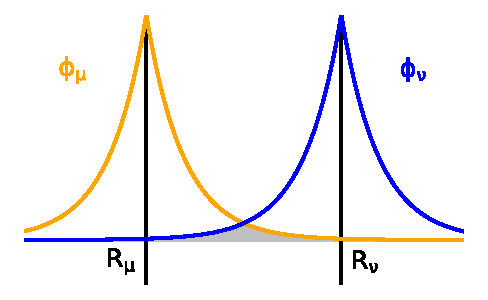
\includegraphics[width=0.5\linewidth]{Figures/Overlap_integral.pdf}
    \caption{Spatial overlap of wavefunctions of two 1s orbitals having the same phase. The atomic orbitals have their origin at R$_{\mu}$ and R$_{\nu}$. The gray shaded area indicates the overlapping area between the two wavefunctions.}
    \label{fig:overlap_integral}
\end{figure}
\noindent
The interaction between two orbitals with each other is quantified in the magnitude of the overlap integral, serving as a powerful tool in the detailed analysis of molecular orbitals. Especially the symmetry of the atomic orbitals is of great importance in dictating whether the overlap integral is zero or not. Figure \ref{fig:symmetry_MOs} shows an overview of various types of overlap integrals. $\sigma$-symmetric orbital overlap is characterized by the absence of nodes along the internuclear axis, whereas $\pi$-symmetric overlap contains a single node, and $\delta$-symmetric contains two nodes along the axis. Nodes along the internuclear axis decrease the overlap between orbitals, which results in a decrease of the overlap integral according to $\sigma > \pi > \delta$. This general rule of thumb is only valid for valence orbitals of atoms from the same row of the periodic table \cite{albright2013orbital} and depends strongly on the spatial extend of the respective atomic orbitals.
\begin{figure}[H]
    \centering
    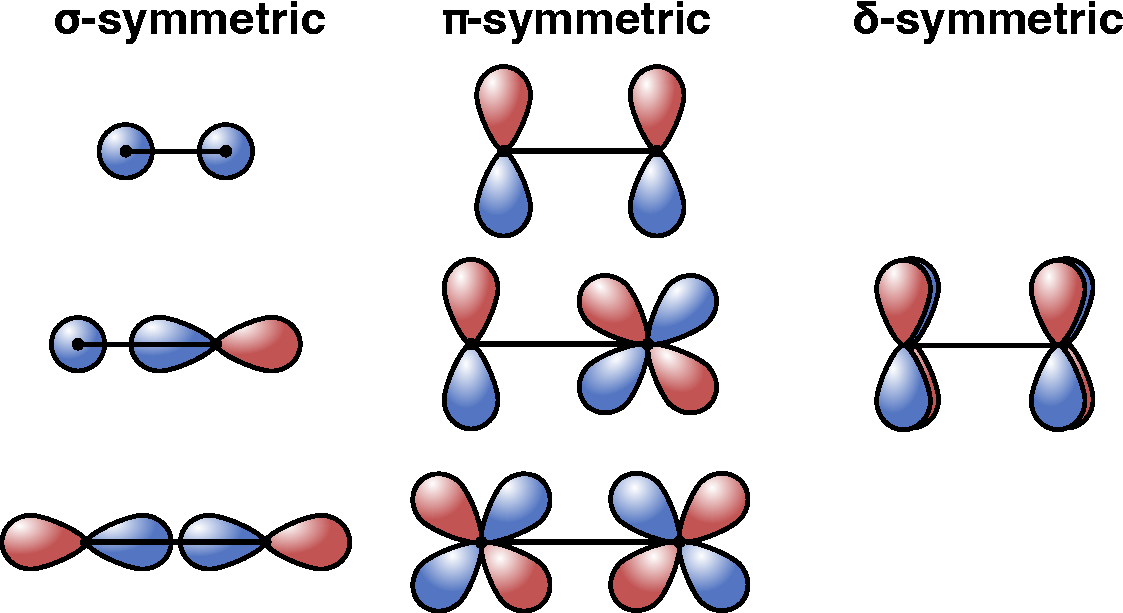
\includegraphics[width=0.8\linewidth]{Figures/Symmetry_orbitals.pdf}
    \caption{Examples of different types of overlap between atomic orbitals. }
    \label{fig:symmetry_MOs}
\end{figure}
\noindent
Another aspect influencing the overlap, is the principle quantum number $n$ of the atomic orbitals. As $n$ increases, the atomic orbitals become more diffuse which normally decreases the overlap. Moreover, the orbital overlap is highly sensitive to the internuclear distance between atoms as well as to the electronegativity, where less electronegative atoms exhibit more diffuse orbitals. An important exception to the generalization discussed above occurs in transition metal complexes. The 3d orbitals are relatively contracted due to their poor radial extension and ineffective shielding by inner electrons. At typical metal-ligand distances, this contraction reduces their spatial overlap with ligand orbitals. In contrast, 4d and 5d valence orbitals are radially more extend as a result of stronger shielding of the positive charge of their nucleus, and therefore exhibit greater overlap with ligand orbitals. Last, the overlap is very sensitive to the geometry of the molecule.
\\Coming back to equation \ref{eq:LCAO_ansatz}, in order to get the optimum value for the orbital coefficients $c$ the variation principle is applied, which leads to the problem of solving the secular equations (an exact derivation can be found here \cite{albright2013orbital}):
\begin{equation}
    \sum_{a} c_{ai}\left(\hat{H}_{\mu\nu}-\epsilon_{i}S_{\mu\nu}\right), 
    \label{eq:secular_equations}
\end{equation}
where $\hat{H}_{\mu\nu}$ is a matrix element of the Hamiltonian and the index $i$ indicates the molecular orbital level. The Hamiltonian is given as:
\begin{equation}
    \hat{H}_{\mu\nu} = \braket{\phi_{\mu}|\hat{H}^{\mathrm{eff}}|\phi_{\nu}}.
    \label{eq:hamiltonina_matrix_element}
\end{equation}
The secular equations \ref{eq:secular_equations} can be express in matrix form as the following:
\begin{equation}
    \textbf{H} \vec{c} = \epsilon \textbf{S}\vec{c}.
    \label{eq:matrix_eigenvalue_problem}
\end{equation}
This is a matrix eigenvalue problem, which represents the formulation of quantum mechanics by Heisenberg. The advantage of this approach is the transformation of differential equations into an algebraic eigenvalue problem, which can be solved efficiently by computer algorithms. Here, \textbf{H} is the Hamiltonian matrix of elements $\hat{H}_{\mu\nu}$, $\vec{c}$ is the coefficient vector containing all unknown orbital coefficients $c_{i}$, $\epsilon$ is the diagonal matrix of energies $\epsilon_{i}$, \textbf{S} is the overlap matrix containing $S_{\mu\nu}$. \\
Solving the eigenvalue equation gives the orbital coefficients and makes the construction of MOs according to LCAO ansatz (see equation \ref{eq:LCAO_ansatz}). For the example of a degenerate interaction, so two atomic orbitals with the same energy, we get the two following MOs:
\begin{align}
    \psi_{1} = \frac{1}{\sqrt{2+2S_{12}}}\left(\phi_{1}+\phi_{2}\right) \\
    \psi_{2} = \frac{1}{\sqrt{2-2S_{12}}}\left(\phi_{1}-\phi_{2}\right)
    \label{eq:MOs_degenerate_interaction}
\end{align}
Here, $\psi_{1}$ is the bonding MO, formed by the in-phase combination of the atomic orbitals $\phi_{1}$ and $\phi_{2}$, whereas $\psi_{2}$ is the anti-bonding MO, formed by the out-of-phase combination. They are depicted in a molecular orbital diagram in Figure \ref{fig:MO_diagrams}a together with the case of nondegenerate interaction (Figure \ref{fig:MO_diagrams}b). The derivation of the analytic expression of those MOs will not be covered here, but can be found in the literature \cite{albright2013orbital}.
\begin{figure}[H]
    \centering
    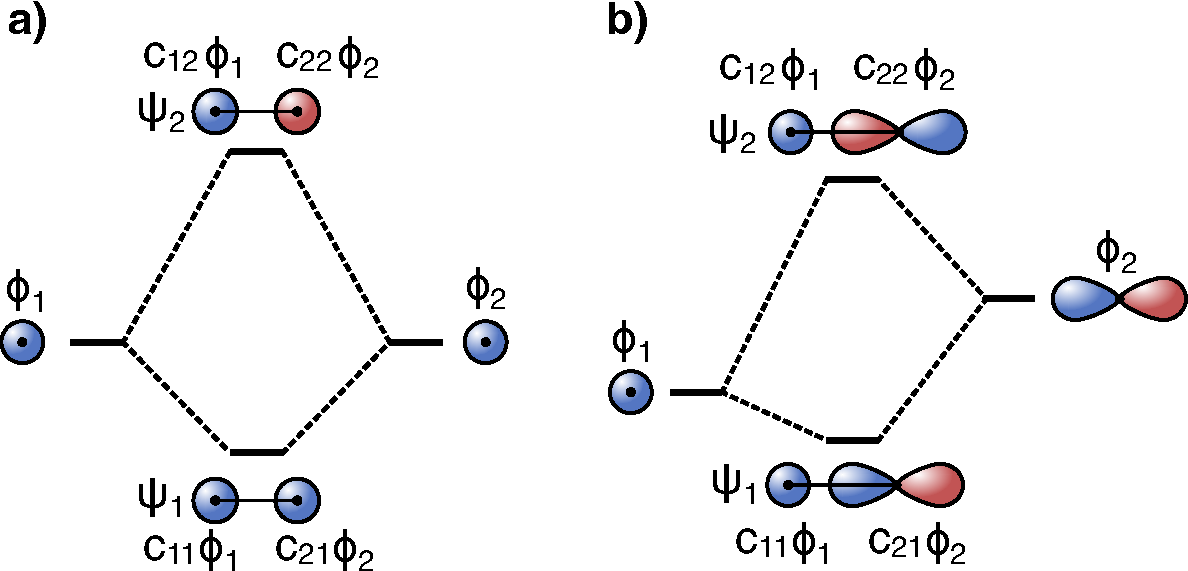
\includegraphics[width=0.95\linewidth]{Figures/MO_diagram_degenreate_and_non_degenerate.pdf}
    \caption{Molecular orbital diagram of a) the degenerate interaction between two atomic s orbitals and b) the non-degenerate interaction between a atomic s and p orbital. The atomic orbitals are denoted as $\phi_{1}$ and $\phi_{2}$ and their in-phase and out-of-phase combination as $\psi_{1}$  and $\psi_{2}$, respectively. The first index of the orbital coefficients indicates the atom and the second the corresponding MO.}
    \label{fig:MO_diagrams}
\end{figure}
\noindent
Until here, we have only considered the two-orbital problem, which is extremely powerful as many bonding situations in chemistry can be reduced into this from. General trends of orbital interactions in this picture can be summarized as the following:
\begin{enumerate}
    \item The upper MO (out-of-phase combination, antibonding) is destabilized more than the lower MO (in-phase combination, bonding).
    \item The magnitude of the interaction energy (MO splitting) increases with increasing overlap of the atomic orbitals.
    \item In nondegenerate orbital interaction, the magnitude of the interaction energy is inversely proportional to the energy difference of the interacting orbitals. The character of a molecular orbital most closely reflects that of the atomic orbital nearest to it in energy.
\end{enumerate}
To get molecular orbitals of polyatomic species, the same LCAO ansatz (see eqauation \ref{eq:LCAO_ansatz} can be utilized with the sum ranging over all atomic molecules of the atoms in the molecule. Similar to the two-orbital example, only atomic molecules with appropriate symmetry can contribute due to their net overlap. \\
With this key concept introduced, we are now able to utilize molecular orbitals to explain the bonding in metal organic complexes, which will be the topic of the next section.

\section{Organometallic Bonding}
\label{sec:Organometallic_Bonding}
Organometallic complexes comprise a vast array of metals, oxidation states, and ligands and thus enable a wide variety of structures and unique bonding motives, which provide the foundation for the reactivity and stability. Thus, it is important to introduce the fundamental principles to understand their unique behavior. We will focus here in particular on organometallic complexes using transition metals. A complete and detailed description of the underlying interactions can be found in the literature \cite{Hartwig_book, albright2013orbital}.
\subsection{Types of Organometallic Bonding}
\label{subsec:types_organometallic_bonding}
In general, a transition metal complex consists of a central transition metal atom which is surrounded by molecules or atoms which are called ligands. An important formalism in organometallic bonding is the determination of the number of electrons of the ligand involved in the bonding to the metal. This interaction are to large extend Lewis acid-base (electron acceptor and donor) interactions, in which the metal often acts as a Lewis acid and the ligand as a Lewis base. This interaction can occur through different modes of orbital overlap between the ligand and metal, with the two most fundamental being $\sigma$-bonding and $\pi$-bonding, which have there name due to the symmetry requirements of the orbitals involved in these interactions (see Figure \ref{fig:symmetry_MOs}). These different bonding motives are schematically shown in Figure \ref{fig:Bonding_in_metal_complexes}.
\begin{figure}[H]
    \centering
    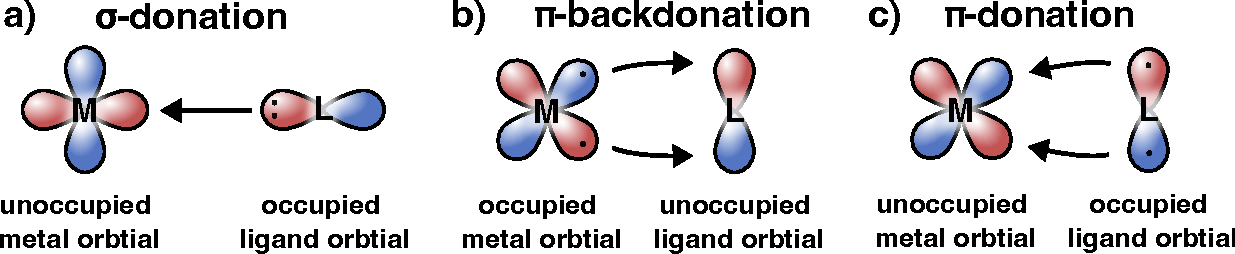
\includegraphics[width=0.95\linewidth]{Figures/Bonding_in_metal_complexes.pdf}
    \caption{Schematic and generalized orbital interactions for a) $\sigma$-donation, b) $\pi$-donation, and c) $\pi$-backdonation in organometallic complexes.}
    \label{fig:Bonding_in_metal_complexes}
\end{figure}
\noindent
In $\sigma$-bonding, the interaction between the ligand and metal arises from the overlap of a filled ligand orbital with metal orbital along the internuclear axis. In most case electron density from a ligand lone pair (e.g. in phosphines or amines) is donates into an empty metal orbital, increasing thereby the electron density at the metal center. Ligands exhibiting such bonding are called $\sigma$-donors. A more special case of $\sigma$-bonding will be discussed in greater detail in section \ref{subsec:sigma_complexes}.\\
In $\pi$-bonded ligands, the involved orbitals of the ligand and metal are oriented perpendicular to the internuclear axis. The interaction between can be divided into $\pi$-donation and $\pi$-back-donation. We focus first on $\pi$-backdonation, in which electron density is transferred from an occupied metal d-orbital into an unoccupied ligand orbital. This interaction is extremely important for the stabilization of complexes with metals in a low formal oxidation states. Most prominent examples for this interaction are carbon monoxide (CO) or nitrosyl cation (NO$^{+}$) which act as strong electron acceptors using their unoccupied $\pi^{*}$-orbitals. This donation of electron density from the metal to the $\pi^{*}$-orbital is know as "backbonding". This destabilizing interaction is more than compensated by the reduced electron density at the metal. In $\pi$-donation, electron density is transferred from an occupied ligand orbital into an empty metal d-orbital, analogous to $\sigma$-donation but involving orbitals oriented perpendicular to the metal-ligand axis. Typical $\pi$-donor ligands are aromatic systems like arenes. In general, these different bonding motives can appear in a single ligand, as long as the symmetry requirements are met for the interactions. However, there relative magnitude is influenced by the electronic structure of the ligand itself. 

\subsection{Sigma-Complexes}
\label{subsec:sigma_complexes}
A special type of metal-ligand interaction occurs in so-called $\sigma$-complexes, in which neutral molecules like dihydrogen, alkanes, silanes and boranes are bound through their H-H, C-H, Si-H or B-H bonds, respectively. Here, we will focus mainly on the case of $\sigma$-alkane complexes as they are the key intermediate in activation of C-H bonds via oxidative addition. The C-H bond binds to the transition metal complex in a combination of two charge transfer interactions (see Figure \ref{} \textcolor{red}{SHOULD I REALLY DO THIS?}), which were first conceptualized on an orbital level by Saillard and Hoffmann \cite{saillard1984carbon}. 
On the one hand, electron density is donated via ligand-to-metal charge transfer (LMCT) from the occupied C-H $\sigma$-orbital to unoccupied metal d-orbitals. On the other hand, electron density is donated in parallel from occupied metal d-orbitals to the unoccupied C-H $\sigma^{*}$-orbital (metal-to-ligand charge transfer, MLCT), acting in the opposite direction. These interactions resemble $\sigma$-donation and $\pi$-backbonding, respectively. The combination of this bidirectional interactions weakens the C-H bond, thereby facilitating C-H activation. Modulation of the metal center's electronic structure plays an important role in enabling the formation of such intermediates and ultimately governs their reactivity in subsequent oxidative addition steps.
\section{Photochemical C-H Activation using Transition Metal Complexes}
\begin{itemize}
    \item examples of C-H activation, small historical back ground
    \item other mechanisms besides C-H activation via sigma complex formation and oxidative addition
    \item reactivity in C-H activation, Hartwig trends, hoffmann sailard explained in detail
\end{itemize}
\textcolor{red}{STILL WRITE THIS STUFF}
    \chapter{Electronic Structure Methods}
\label{chapter:Electronic_Structure_Methods}
In the previous chapter, the general concept of MO theory was introduced, which allows the understanding of chemical bonding based on its electronic structure. Until here, the exact energy of these orbitals has been only partially covered. In order to change this, theoretical electronic structure methods are introduced to calculate those energies, which enable us to calculate spectra allowing for comparison with experimental observables. The equations are taken from literature textbooks \cite{szabo1996modern, jensen2017introduction}, which describe their derivation in greater detail.

\section{Hartree-Fock Methods}
\subsection{The Electronic Hamiltonian}
\label{sec:Hartree_Fock}
The basis of calculating the energy of a system is the Schr\"odinger equation (eq. \ref{eq:Schroedinger_equation} introduced in section \ref{sec:MO_theory}, consisting of the Hamiltonian $\hat{H}$ and the wavefunction $\Psi$. Until here, only the general form of the Hamiltonian has been introduced in equation \ref{eq:Hamilton_operator}, which can be further dissected into kinetic and potential energies of the nuclei and electrons:
\begin{equation}
    \hat{H} = \hat{T}_{e} + \hat{T}_{N} + \hat{V}_{ee} + \hat{V}_{eN} + \hat{V}_{NN},
    \label{eq:Hamilton_operator_expaneded}
\end{equation}
where $\hat{T}$ and $\hat{V}$ are the operators for kinetic and potential energy for electrons $e$ and nuclei $N$. Thus the terms $ \hat{V}_{eN}, \hat{V}_{ee}$, and $\hat{V}_{NN}$ describe the electron-nuclei attraction, electron-electron repulsion and nuclei-nuclei repulsion, respectively. This Hamiltonian provides a formally exact description, however solving the corresponding Schr\"odinger equation is intractable due to the simultaneous treatment of all particles. A key approximation to circumvent this issue is the Born-Oppenheimer approximation \cite{born_oppenheimer1927}. As nuclei are much heavier than electrons, they move more slowly. Thus it can be assumed that electrons move in a field of fixed nuclei. Within this approximation, the kinetic energy operator for nuclei $\hat{T}_{N}$ can be neglected and the nuclei-nuclei repulsion $\hat{V}_{NN}$ can be considered to be constant. The remaining terms of equation \ref{eq:Hamilton_operator_expaneded} are summarized as the electronic Hamiltonian $\hat{H}_{elec}$ and can be written as the following in its operator form:
\begin{equation}
    \hat{H}_{elec} = \underbrace{-\sum_{i = 1}^{A}\frac{1}{2}\nabla^{2}_{i}}_{\hat{T}_{e}}  + \underbrace{\sum_{i=1}^{A}\sum_{j>i}^{A}\frac{1}{r_{ij}}}_{\hat{V}_{ee}}  \underbrace{-\sum_{i=1}^{A}\sum_{N=1}^{B}\frac{Z_{N}}{r_{iN}}}_{\hat{V}_{eN}}.
    \label{eq:Hamilton_operator_electronic}
\end{equation}
Here, $\nabla^{2}$ is the Laplace operator, $r_{ij}$ is the distance between the electrons $i$ and $j$, $r_{ij}$ is the distance between electron $i$ and nucleus $N$ with its atomic number $Z_{N}$. Solving the Schr\"odinger equation for the electronic Hamiltonian, yields the electronic energy as a function of the position of the nuclei $E_{elec}(R)$ (potential energy surface), on which the nuclei move. The total energy $E_{tot}$ can then be calculated by adding the $V_{NN}$ term afterwards, as it has not direct influence on the wavefunction. This assumption directly introduces the adiabatic approximation, which assumes that the nuclear dynamics remain confined to a single electronic state, neglecting couplings to different states. As a consequence no electronic surface transitions are possible.

\subsection{The "Correct" Wavefunction}
In the previous chapter we have manly focused on the one-electron wavefunctions which give access to molecular orbitals of a system. In this chapter, we will take a step back and reconsider what the correct choice of the wavefunction is to describe systems using the Schr\"odingner equation. The basis for construction of the many-electron wavefunction is the LCAO ansatz introduced in section \ref{sec:MO_theory}, which allows the construction of molecular orbitals on the basis of atomic basis functions. One approach for these atomic basis functions are so-called Slater functions, which are the solutions of the H atom. They are of the type:
\begin{equation}
   \phi = Y_{l}^{m}(\theta, \phi) \cdot r^{n-1}\mathrm{exp}\frac{-\zeta\cdot |r|}{n},
    \label{eq:Slater_function}
\end{equation}
where $Y_{l}^{m}(\theta, \phi)$ are the spherical harmonics, $n, l, m$ are the quantum numbers, and $\zeta$ is a constant related to the effective charge of the nucleus. However, their integration is very expensive and numerically problematic. Thus, other easier to integrate functions need to be utilized. For molecules, the solution is to use spherical Gaussian functions of the form:
\begin{equation}
   \phi = Y_{l}^{m}(\theta, \phi) \mathrm{exp}(-\zeta\cdot r^2).
    \label{eq:spherical_Gaussian_function}
\end{equation}
In contrast to Slater functions, calculations using Gaussian is computational inexpensive (Gaussian product theorem) and the integrals involving them can be solved analytically. Their main drawback is the wrong description of the short- and long-range behavior (to low intensity close to the nucleus and to low intensity at large distances from the nucleus). The solution to this, are so-called contracted Gaussians type orbitals (CGTOs), which are a linear combination of typical 2 to 10 primitive Gaussians type orbitals (PGTOs):
\begin{equation}
   \phi^{\mathrm{CGTO}} = \sum_{i}^{\approx2-10} c_{i}\phi_{i}^{\mathrm{PGTO}}(\zeta_{i})
    \label{eq:contracted_Gaussians}
\end{equation}
Until here, the approaches were only solutions for one-electron wavefunctions. The simplest approximation to approach many-electron systems is the so-called Hartree ansatz, which gives the wavefunction of a many-electron system as a combination of individual one electron functions (also called Hartree product) which is given as:
\begin{equation}
   \Psi^{\mathrm{HP}} = \phi_{1}(1)\phi_{2}(2)\cdots \phi_{N}(N),
    \label{eq:Hartree_product}
\end{equation}
for an $N$-electronic systems with each electron in their individual state. In the Hartree product, the electrons are treated as independent particles that interact only through an average or "mean-field" potential generated by the presence of all other electrons. We will return to this issue later in the chapter. Beyond this mean-field approximation, the Hartree product suffers from two additional shortcomings. First, because the electrons are explicitly assigned to specific orbitals, the wavefunction does not satisfy the required antisymmetry condition for fermions (particles with a spin = $n + \frac{1}{2}$). Second, this formulation incorrectly renders the electrons distinguishable, whereas they are fundamentally indistinguishable particles. The indistinguishability and antisymmetry of electrons is implemented by expression of the wavefunction as a Slater determinant:
\begin{equation}
\Psi^{\mathrm{SD}} = \frac{1}{\sqrt{N!}}
\begin{vmatrix}
\phi_{1}(1) & \phi_{1}(2) &  \cdots & \phi_{1}(N) \\ 
\phi_{2}(1) & \phi_{2}(2) &  \cdots & \phi_{2}(N) \\
\vdots &  \vdots & \ddots &\vdots \\
\phi_{N}(1) & \phi_{N}(2) &  \cdots & \phi_{N}(N)\\ 
\end{vmatrix}\\
= \ket{\phi(1)\phi(2)\cdots\phi(N)}
\end{equation}

\subsection{The Hartree-Fock Procedure}
\label{sec:The_Hartree-Fock_Procedure}
With now a valid wavefunction and Hamiltonian, we can now proceeding to calculate the energy of a system. As discussed previously, an exact solution to the Schr\"odinger equation can only be obtained for one-electron systems. For many-electron systems, approximate solutions must be employed. One approach is based on the variational principle, which states that every approximate solution of the wavefunction possesses an energy which always exceeds the exact energy $E_{0}$. This approximate energy can be optimized by iteratively trying to minimize the energy by optimizing the orbitals (one-electron wavefunctions) which are used to construct the many-electron wavefunction. In order to do so, we need to transform the Schr\"odinger equation into a matrix eigenvalue problem, which can iteratively be solved in computer algorithms. \\
The first step is the dissection of the electron Hamiltonian (see eq. \ref{eq:Hamilton_operator_electronic}) into one-electron $\mathcal{O}_{1}$ ($\hat{T}_{e}$ and $\hat{V}_{eN}$) and two-electron $\mathcal{O}_{2}$ ($\hat{V}_{ee}$) operators. For the one-electron operators, integration is performed only over the orbitals associated with the $i$-th electron, while contributions from all other orbitals vanish due to their integrals resulting to unity. The two one-electron operators are often combined into a single operator, denoted as $h$. The two-electron operator can be further decomposed into the Coulomb integral $J_{ij}$, which describes the classical Coulomb repulsion between two electrons $i$ and $j$, and the exchange integral $K_{ij}$, which has no classical analogue. The exchange integral arises purely from quantum mechanics, as a consequence of the indistinguishability of fermions and the antisymmetry requirement of the wavefunction. This phenomenon can be understood as follows: Each electron creates an exchange hole in its vicinity, a region from which other electrons of the same spin are excluded. This behavior is a manifestation of the Pauli-Principle. A detailed derivation of these terms can be found here \cite{jensen2017introduction}. Using these new integrals the energy of a Slater determinant can be written as:
\begin{equation}
    E_{elec} = \sum_{i}^{A}h_{i} \sum_{i<j}^{A, A} J_{ij} - K_{ij}
    \label{eq:Energy_Slater}
\end{equation}
According to this equation, each electron contributes an attraction to the nuclei and possesses a certain kinetic energy, both described by the one-electron operator $h$. Furthermore, each unique pair of electrons contributes a Coulomb repulsion term $J$, which is subsequently corrected by the exchange interaction $K$ for pairs of electrons with the same spin. For the purpose of deriving at an expression to be used in the variational principle, it is convenient to transform the energy expression in \ref{eq:Energy_Slater} in terms of its operator form, which is called the Fock operator:
\begin{equation}
    f(1) = h(1) + \sum_{i}^{A}\mathcal{J}_{i}(1)-\mathcal{K}_{i}(1).
    \label{eq:fock_operator}
\end{equation}
This new one-electron operator obtains a set of $A$ (number of electrons) interdependent eigenvalue problems: 
\begin{equation}
    \left\{
    f(i)\psi_{i}(i) = \epsilon_{i} \cdot \psi_{i}(i) \right\}.
    \label{eq:Fock_eignevalues}
\end{equation}
Using the definition of the molecular orbitals via the LCAO ansatz (see equation \ref{eq:LCAO_ansatz}) and inserting it into equation \ref{eq:Fock_eignevalues} we yield:
\begin{equation}
    f(i)\sum_{a}^{M_{basis}}c_{ai}\phi_{a} = \epsilon_{i}\sum_{a}^{M_{basis}}c_{ai}\phi_{a},
    \label{eq:Fock_eignevalues_plugged_in}
\end{equation}
where $M_{basis}$ is the amount of atom centered basis functions. Multiplying from the left by a specific basis function and integrating yields the Roothaan-Hall equations \cite{RevModPhys.23.69}. These are the Hartee-Fock equations in the atomic orbital basis. They can be collected for all $M_{basis}$ equations in a matrix notation:
\begin{equation}
    \textbf{FC} = \textbf{SC}\epsilon, 
    \label{eq:Hartree_fock_equation_matrix}
\end{equation}
with 
\begin{equation}
    \textbf{F}_{\mu\nu} = \braket{\phi_{\mu}|f(1)|\phi_{\nu}} \qquad \mathrm{and} \qquad \textbf{S}_{\mu\nu} = \braket{\phi_{\mu}|\phi_{\nu}}
    \label{eq:Fock_matrix}
\end{equation}
\subsection{Post Hartree-Fock Methods}
\label{sec:Post_Hartree-Fock_Methods}

\section{Density Functional Theory}
\label{sec:DFT}
Write some stuff about DFT here
    \chapter{X-ray Based Spectroscopy Methods}
\label{chapter:X-ray_Based_Spectroscopy_Methods}
In this chapter, the theoretical basics behind X-ray absorption spectroscopy (XAS) and resonant inelastic X-ray scattering (RIXS), which are the main experimental techniques used in this thesis, will be investigated. Both techniques can be used to investigate the local, element specific, electronic structure. This is of great advantage in comparison to conventional electronic spectroscopies like UV/Vis where the signals are broad and overlap with solvent bands, making it difficult to attribute them to distinct orbital contributions.
\section{Quantum Formulation of X-ray Interactions with Matter}
\label{sec:X-ray_Interaction_with_Matter}
X-rays interact with matter in through a variety of processes, each of them having different purposes in research or medical applications. Here, we will focus only on the interaction leading to X-ray absorption as this is the underlying process in the experimental techniques used in this thesis. This process involves an excitation of a core electron through the energy transfer of a photon to a bound electron, which is better known as the photoelectric effect \textcolor{red}{CITATION}. To calculate and understand the underlying transitions of this process, the quantum mechanical description of this interaction will be discussed in the following section.
\subsection{Basic Premise}
The quantum mechanical description of the photon-matter interactions has its roots in a paper by Kramers and Heisenberg in 1925 \cite{kramers1925streuung}, written just prior to the formal establishment of quantum theory. Their central idea was that the interaction between photons and matter can be treated as a weak perturbation of the matter's equilibrium state \cite{stohr2023nature}. As a results, photons act as a probe of the unperturbed ground state of matter. To model this perturbation, a Hamiltonian is required describing the interaction of an electromagnetic field with the electron charge and spin.  A derivation of the complete interaction Hamiltonian can be found in the literature \cite{stohr2023nature}. For simplicity, we consider only the most dominant terms which are given as:
\begin{equation}
    \hat{H}_{int} = \underbrace{\frac{e^{2}}{2m_{e}}\hat{A}^{2}}_{\substack{\text{Thomson}\\\text{scattering}}}
    +\underbrace{\frac{e}{m_{e}}\hat{p}\cdot\hat{A}}_{\substack{\text{photoelectric}\\\text{transitions}}} , 
    \label{eq:tot_hamiltonian}
\end{equation}
where $e$ is the elementary charge, $m_{e}$ the electron mass, $\hat{A}$ is the time-dependent vector potential and $\hat{p}$ the momentum, given in operator form. The vector potential $\hat{A}(\textbf{r},t) = \hat{A}^{ab} + \hat{A}^{em}$ can cause absorption (and thereby photon destruction) or emission (through photon creation) \cite{stohr2023nature}. If the term depends linearly on $\hat{A}$, it describes processes in which a photon is either created or annihilated, but not both simultaneously. In contrast, if the term depends quadratically on $\hat{A}$, it allows for both photon creation and annihilation, corresponding to scattering processes. \\
The essence of the description of electronic excitations lies in the assumption that the system is mostly time independent and that the time evolution can be approximate by a weak perturbation. This concept is used in time-dependent perturbation theory where the total Hamiltonian can be separated into two parts $\hat{H} = \hat{H}_{0} + \hat{H}'$ where the  $\hat{H}'$ acts a weak time-dependent perturbation of the stationary $\hat{H}_{0}$. This is justified here as the interaction process with a single photon is so fast (<\SI{1}{\atto\second}) that it is not affected by other atomic effects witch occur on longer timescales. This relative speed comparison is the same concept as in the Born-Oppenheimer approximation \cite{born_oppenheimer1927}. Using the quantization of the electromagnetic field introduced by Dirac in 1927 \cite{dirac1927quantizationEM}, this leads to the Kramers-Heisenberg-Dirac perturbation theory.
\subsection{The Kramers-Heisenberg-Dirac Formula}
According to the Kramers-Heisenberg-Dirac (KHD) perturbation theory, the time-dependent electromagnetic field induces a transitions from an initial state $\ket{i}$ to a final state $\ket{f}$. Both states include electronic and photonic components, and the transition can be envisioned as proceeding through a multiple steps. First, the electronic and photon parts of the system are decoupled, so that the electronic ground state evolves according to the time-independent Hamiltonian. Second, the interaction takes place, when the electronic state is perturbed by the interaction Hamiltonian $\hat{H}_{int}$ (see eq. \ref{eq:tot_hamiltonian}) generating a new state $\ket{f}$. This transition can be written as $\braket{f|\hat{H}_{int}|i}$. Third, the electronic excited state evolves again according to the time-independent Hamiltonian. In second order, the transition is made through an intermediate state $m$, which gives $\braket{f|\hat{H}_{int}|m}\braket{m|\hat{H}_{int}|i}$. The analogue formulation can be made for higher order of perturbations, however we stop here after the second order term, which can be then formulated as the Kramers-Heisenberg-Dirac (KHD) formula, which is the starting point of quantitative calculation of electronic X-ray processes under the assumption of the Born-Oppenheimer approximation \cite{stohr2023nature}. The transition probability $\mathcal{W}_{if}$ from a state $i$ to a state $f$ is given as:
\begin{equation}
    \mathcal{W}_{if} = \frac{2\pi}{\hbar}\left|\underbrace{\braket{f|\hat{H}_{int}|i}}_{1^{st}}+\underbrace{\sum_{m}\frac{\braket{f|\hat{H}_{int}|m}\braket{m|\hat{H}_{int}|i}}{\mathcal{E}_{i}-\mathcal{E}_{m}}}_{2^{nd}}\right|^{2} \rho\left(\mathcal{E}_{f}\right)\delta\left(\mathcal{E}_{f}-\mathcal{E}_{i}\right),
    \label{eq:Kramers-Heisenberg-Dirac}
\end{equation}
where $\hat{H}_{int}$ is the interaction Hamiltonian, $\ket{i}$, $\ket{m}$ and $\ket{f}$ are the wavefunctions of the initial, intermediate and final state with their respective energies $\mathcal{E}_{i}$, $\mathcal{E}_{m}$ and $\mathcal{E}_{f}$, $\rho(\mathcal{E}_{f})$ is the density of states of final states, and $\delta$ is the Dirac $\delta$-function conserving the energy. The first term of the matrix element is better known as "Fermi's golden rule" \cite{fermi1932}. The second term describes transitions from the initial state $i$ to the finale state $f$ over a range of possible intermediate states $m$. Based on this equation, we will discuss in the following sections the transition rate and cross-sections of the processes in X-ray absorption spectroscopy and Resonant inelastic X-ray scattering.
\begin{figure}[H]
    \centering
    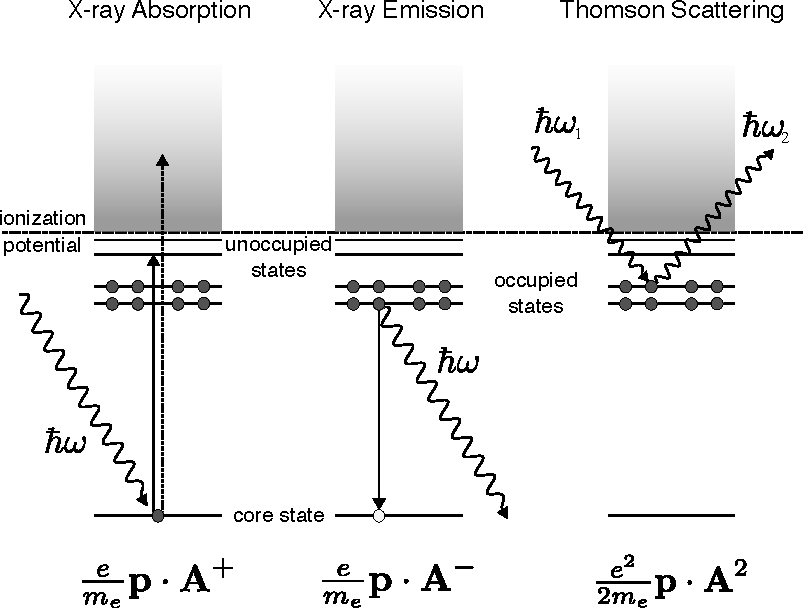
\includegraphics[width=0.8\linewidth]{Figures/first_order_interaction_processes.pdf}
    \caption{Schematic of the first order quantum mechanical process upon interaction of X-rays with matter. Electrons are shown as filled circles, holes as open circles. The operators for the processes are shown below.}
    \label{fig:Overview_first_order_processes}
\end{figure}
\noindent
Using only the first order term of the KHD equation (eq. \ref{eq:Kramers-Heisenberg-Dirac}), leads to the quantum mechanical description of X-ray absorption, X-ray emission and X-ray Thomson scattering, illustrated in Figure \ref{fig:Overview_first_order_processes}, along with their respective interaction Hamiltonian. In X-ray absorption or emission the X-ray photon is absorbed (destroyed) or emitted (created). This is described by the destruction operator $\hat{A}^{+}$ or the creation operator $\hat{A}^{-}$, respectively. Thomson scattering does neither destroys or creates photons and can occur as an elastic or inelastic process. In the following, we will discuss the underlying concepts of X-ray absorption in greater detail.
\section{X-ray Absorption Spectroscopy}
The strongest interaction of X-rays with matter is X-ray absorption. In this process, the incident electric field couples to a core electron, resulting in the absorption of the photon and the transfer of its energy to the electron, which is thereby promoted to an unoccupied level or ejected from the system if the incidence energy is larger than the ionization potential. Both processes are depicted in Figure \ref{fig:Overview_first_order_processes} (solid and dashed line). Measuring the photon energy dependent cross section, which is the sum of all photoemission cross sections of orbitals with energy lower than the photon energy, is the main essence of X-ray absorption spectroscopy (XAS). This cross section changes smoothly with photon energy, decreasing with increasing photon energy (shell specific photoemission cross section increases with photon energy), and exhibits sharp so-called absorption edges, where the photon energy matches resonant excitations.
\begin{figure}[H]
    \centering
    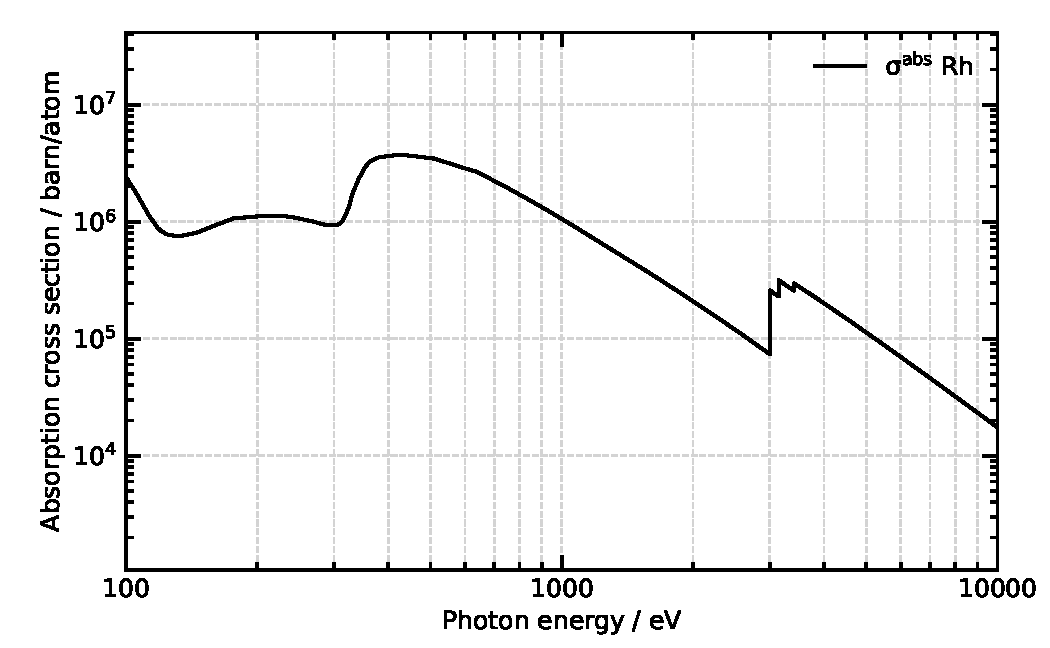
\includegraphics[width=\linewidth]{Figures/Cross_section_Rh.pdf}
    \caption{Energy dependent X-ray absorption cross section for Rh. The cross sections were calculated from atomic scattering factors from literature \cite{henke1993x}.}
    \label{fig:Rh_Cross_section}
\end{figure}
\noindent
Excitations which exceed resonance excitations in energy can arise from multi-electron excitations, and in the case of molecular or condensed matter due to back scattering of photoelectrons from neighboring atoms. This part of the spectrum is called extended X-ray absorption fine structure (EXAFS) and will not be discussed here in detail. We will focus here on the resonant near absorption fine structure (NEXAFS) part of XAS, which corresponds to excitations of core electrons to empty valence orbitals, which makes it sensitive to the bonding environment. \\\
To get back to the quantum mechanical description, we utilized the first order term of the KHD equation (\ref{eq:Kramers-Heisenberg-Dirac} which gives the transition rate for X-ray absorption:
\begin{equation}
    \mathcal{W}_{if}^{abs} = \frac{2\pi}{\hbar}\left|\braket{f|\hat{H}_{int}|i}\right|^{2} \rho\left(\mathcal{E}_{f}\right)\delta\left(\mathcal{E}_{f}-\mathcal{E}_{i}\right).
    \label{eq:XAS_transition_rate}
\end{equation}
with $\hat{H}_{int} = e \textbf{r}\cdot\hat{E}$, which is a combination of the dipole operator $e\ \textbf{r}$ and the field operator $\hat{E}$ which can analogously to vector potential $\hat{A}$ can destroy ($\hat{E}^{+}$) or create ($\hat{E}^{-}$) photons. Until here, the electric field operator $\hat{E}$ depends on the wave vector \textbf{k}, according to  
\begin{equation}
    E(\textbf{r}, t) = E_{0}e^{i\left(\textbf{k}\cdot\textbf{r}-\omega t\right)},
    \label{eq:electric_field}
\end{equation}
where $\textbf{r}$ is the position vector, $\omega$ is the angular frequency and $t$ is the time. In the dipole approximation, the exponential can be expanded as 
\begin{equation}
   e^{i\textbf{k}\cdot\textbf{r}} = 1 + i\textbf{k}\cdot\textbf{r} + \cdots \simeq 1, 
    \label{eq:exponential_expansion}
\end{equation}
which makes the electric field uniform across the interaction region. As a result, the interaction Hamiltonian $\hat{H}_{int}$ reduces to the dipole operator, and dipole-allowed transitions -- subject to the selection rule $\Delta L = \pm 1$ -- dominate the transitions. To get the cross section for the X-ray absorption process, the transition rate per unit time $\mathcal{W}_{if}^{abs}$ has to be normalized by the incident photon flux $\Phi_{0}$
\begin{equation}
    \sigma^{abs} = \frac{\mathcal{W}_{if}^{abs}}{\Phi_{0}} \qquad \mathrm{with} \qquad \Phi_{0}=\frac{c n_{0}}{V}=\frac{2\epsilon_{0}cE^{2}_{0}}{\hbar\omega},
    \label{eq:XAS_cross_section}
\end{equation}
where $\epsilon_{0}$ is the electric field constant, $c$ the speed of light and $E_{0}$ the amplitude of the electric field. The photon flux $\Phi$ can be imagined as the number of photons $n_{0}$ flowing with the speed of light $c$ through a specific volume $V$.\\
Following the creation of a core hole through photon absorption, the system stabilizes by spontaneously filling the vacancy. The core hole is filled by an electron form a higher energy level which results in the release of energy. This energy can be either transferred to a valence electron which is ejected from the atom (Auger-Meitner decay) or by the emission of a photon (fluorescence). The ratio of these two decay channels varies with the atomic number $Z$, with Auger-Meitner decay being favored for lighter elements and fluorescence for heavier elements \cite{kotani2001resonant}. The final states reached through these two channels are distinct, meaning that they do not interfere. Consequently, the individual decay rates for X-ray emission $\Gamma^{X}$ and for Auger-Meitner decay $\Gamma^{AM}$ can be summed to give total decay rate $\Gamma$:
\begin{equation}
    \Gamma = \Gamma^{X} + \Gamma^{AM}
    \label{eq:decay_rate_XAS}
\end{equation}
The finite lifetime of the electronic excited states results in a natural broadening, also known as lifetime broadening. This is a result of the Heisenberg uncertainty principle \cite{heisenberg1927anschaulichen}, which, in its energy-time relation, refers the lifetime to its uncertainty in energy
\begin{equation}
    \Delta E \Delta t \geq  \frac{\hbar}{2},
    \label{eq:Heisenberg_uncertainty}
\end{equation}
where $\Delta E$ is the uncertainty in energy and $\Delta t$ is the uncertainty in time. As the decay of electronic excited state occurs exponentially in time, the corresponding lineshape are Lorentzian and $\Gamma$ represents the Lorentzian FWHM. 
\section{Resonant Inelastic X-ray Scattering}

\section{Time-resolved Spectroscopy}
\section{X-ray Sources}
\label{sec:X-ray_sources}
\subsection{Synchrotron Radiation}
\subsection{Free Electron Lasers}

    \chapter{Results}

\section{Paper I: Time-resolved Resonsant Inelastic X-ray Scattering reveals how Molecular Orbital Symmetry Alignment enables C-H Activation with Cp*Rh(CO)$_{2}$ and CpRh(CO)$_{2}$}

% \section{Ultrafast Dynamics of Rh(acac)(CO)\texorpdfstring{$_{2}$}{2} in Acetonitrile solution Probed by Time-Resolved X-ray Absorption Spectroscopy}

% \section{CpCO(CO)2 in octane}

% \section{Ultrafast Dynamics of Cp*Ir(CO)\texorpdfstring{$_{2}$}{2}, CpIr(CO)\texorpdfstring{$_{2}$}{2} and Ir(acac)(CO)\texorpdfstring{$_{2}$}{2} Probed by Time-Resolved UV/Vis and X-ray absorption spectroscopy}
    \chapter{Discussion and Outlook}


\backmatter
    % References
    % No restriction is set to the reference styles
    % Save your references in References.bib
    \nocite{*} % Remove this for your own citations
    \bibliographystyle{unsrt}
    \bibliography{References}

\end{document}